\documentclass[../differential_methods.tex]{subfiles}
\begin{document}
\section{Aula 08 - 08 de Abril, 2026}
\subsection{Motivações}
\begin{itemize}
	\item Problemas de Valor Inicial.
\end{itemize}
\subsection{Problemas de Valores Iniciais: método de Euler}
Vários fenômenos físicos são modelados por equações diferenciais ordinárias, ou sistemas delas. Assim, temos um grande interesse em resolver problemas de valores iniciais (doravante PVIs), que costumam modelar fenômenos físicos de evolução ao longo do tempo.
Mais exatamente, seja \(f:\Omega \times [0,T]\rightarrow \mathbb{R}^{m}\), com \(\Omega \subseteq \mathbb{R}^{m},\; m\geq 1\) e \([0, T]\subseteq \mathbb{R}\); procuramos uma função \(u:[0,T]\rightarrow \mathbb{R}^{m}\) tal que
\[
	\frac{\mathrm{d}}{\mathrm{d}t}u(t)\eqqcolon u'(t) = f(u(t), t),\quad \forall t\in [0,T]
\]
e \(u(0)=u_{0}\) é a condição inicial conhecida.

\begin{example}[Equação Escalar]
	Um exemplo de equação escalar é
	\[
		y'=x^{2}+y^{2},\quad y(0)=0.5,
	\]
	que está na forma \(y'(x)=f(y(x), x)\), onde
	\[
		f(y(x), x)=x^{2}+y^{2}.
	\]
\end{example}
\begin{example}[Modelo Presa-Predador de Lotka-Volterra]
	Este modelo descreve a dinâmica entre duas populações, uma denominada predador (u) e outra denominada presa:
	\[
		\left\{\begin{array}{ll}
			u'(t)=-2u + uv \\
			v'(t)=v-uv     \\
			u(0)=u_{0}     \\
			v(0)=v_{0}
		\end{array}\right.,
	\]
	resultando nas expressões
	\begin{align*}
		 & \tikz[baseline=-0.5ex]\draw[black, fill=black, radius=1.5pt](0, 0)circle;\; \mathbf{u}(t)=\begin{bmatrix}
			                                                                                             u_1(t) \\
			                                                                                             u_2(t)
		                                                                                             \end{bmatrix} = \begin{bmatrix}
			                                                                                                             u(t) \\
			                                                                                                             v(t)
		                                                                                                             \end{bmatrix};         \\
		 & \tikz[baseline=-0.5ex]\draw[black, fill=black, radius=1.5pt](0, 0)circle;\; \mathbf{u}_{0}= \begin{bmatrix}
			                                                                                               u_{0} \\
			                                                                                               v_{0}
		                                                                                               \end{bmatrix};                       \\
		 & \tikz[baseline=-0.5ex]\draw[black, fill=black, radius=1.5pt](0, 0)circle;\; \mathbf{f}(\mathbf{u}(t), t) = \begin{bmatrix}
			                                                                                                              -2u_1(t)+u_1(t)u_2(t) \\
			                                                                                                              u_2(t)-u_1(t)u_2(t)
		                                                                                                              \end{bmatrix},
	\end{align*}
	tais que podemos escrever
	\[
		\left\{\begin{array}{ll}
			\mathbf{u}'(t)=\mathbf{f}(\mathbf{u}(t), t) \\
			\mathbf{u}(0)=\mathbf{u}_{0}
		\end{array}\right.
	\]
\end{example}
\begin{example}[Pêndulo]
	A dinâmica de um pêndulo ideal sob ação da gravidade é modelado por um sistema de equações diferenciais de ordem 2:
	\[
		\left\{\begin{array}{ll}
			q''=-\sin^{}{q} \\
			q(0)=q_{0}      \\
			q'(0)=p_{0}
		\end{array}\right. \Rightarrow \left\{\begin{array}{ll}
			q'=p           \\
			p'=-\sin^{}{q} \\
			q(0)=q_{0}     \\
			p(0)=p_{0}
		\end{array}\right.,
	\]
	que leva às expressões para a forma usual dadas por:
	\begin{align*}
		 & \tikz[baseline=-0.5ex]\draw[black, fill=black, radius=1.5pt](0, 0)circle;\; \mathbf{u}(t)=\begin{bmatrix}
			                                                                                             u_1(t) \\
			                                                                                             u_2(t)
		                                                                                             \end{bmatrix} = \begin{bmatrix}
			                                                                                                             q(t) \\
			                                                                                                             p(t)
		                                                                                                             \end{bmatrix};                             \\
		 & \tikz[baseline=-0.5ex]\draw[black, fill=black, radius=1.5pt](0, 0)circle;\; \mathbf{u}_{0}= \begin{bmatrix}
			                                                                                               q_{0} \\
			                                                                                               p_{0}
		                                                                                               \end{bmatrix};                                           \\
		 & \tikz[baseline=-0.5ex]\draw[black, fill=black, radius=1.5pt](0, 0)circle;\; \mathbf{f}(\mathbf{u}(t), t) = \begin{bmatrix}
			                                                                                                              u_2(t) \\
			                                                                                                              -\sin^{}{u_{1}(t)}
		                                                                                                              \end{bmatrix}.
	\end{align*}
\end{example}
\begin{example}[Gravitação]
	A dinâmica de um objeto de massa desprezível girando em torno do sol é dada pelo sistema de ordem 4 abaixo:
	\[
		\left\{\begin{array}{ll}
			\frac{\mathrm{d}^{2}x}{\mathrm{d}t^{2}} =-\frac{x}{(x^{2}+y^{2})^{\frac{3}{2}}} \\
			\frac{\mathrm{d}^{2}y}{\mathrm{d}t^{2}}=-\frac{y}{(x^{2}+y^{2})^{\frac{3}{2}}}  \\
			x(0)=x_{0},\; y(0)=y_{0}                                                        \\
			x'(0)=u_{0},\; y'(0)=v_{0}
		\end{array}\right. \Rightarrow \left\{\begin{array}{ll}
			\frac{\mathrm{d}x}{\mathrm{d}t}=u                                       \\
			\frac{\mathrm{d}u}{\mathrm{d}t}=- \frac{x}{(x^{2}+y^{2})^{\frac{3}{2}}} \\
			\frac{\mathrm{d}y}{\mathrm{d}t}=v                                       \\
			\frac{\mathrm{d}v}{\mathrm{d}t}=-\frac{y}{(x^{2}+y^{2})^{\frac{3}{2}}}  \\
			x(0)=x_{0},\; y(0)=y_{0}                                                \\
			x'(0)=u_{0},\; y'(0)=v_{0}
		\end{array}\right.,
	\]
	com expressões usuais
	\begin{align*}
		 & \tikz[baseline=-0.5ex]\draw[black, fill=black, radius=1.5pt](0, 0)circle;\; \mathbf{u}(t)=\begin{bmatrix}
			                                                                                             u_1(t)   \\
			                                                                                             u_2(t)   \\
			                                                                                             u_{3}(t) \\
			                                                                                             u_{4}(t)
		                                                                                             \end{bmatrix} = \begin{bmatrix}
			                                                                                                             x(t) \\
			                                                                                                             u(t) \\
			                                                                                                             y(t) \\
			                                                                                                             v(t)
		                                                                                                             \end{bmatrix};                                                 \\
		 & \tikz[baseline=-0.5ex]\draw[black, fill=black, radius=1.5pt](0, 0)circle;\; \mathbf{u}_{0}= \begin{bmatrix}
			                                                                                               x_{0} \\
			                                                                                               u_{0} \\
			                                                                                               y_{0} \\
			                                                                                               v_{0}
		                                                                                               \end{bmatrix};                                                               \\
		 & \tikz[baseline=-0.5ex]\draw[black, fill=black, radius=1.5pt](0, 0)circle;\; \mathbf{f}(\mathbf{u}(t), t) = \begin{bmatrix}
			                                                                                                              u_2(t)                                             \\
			                                                                                                              -\frac{u_{1}}{(u_{1}^{2}+u_{3}^{2})^{\frac{3}{2}}} \\
			                                                                                                              u_4(t)                                             \\
			                                                                                                              -\frac{u_{3}}{(u_{1}^{2}+u_{3}^{2})^{\frac{3}{2}}}
		                                                                                                              \end{bmatrix}.
	\end{align*}
\end{example}
\begin{example}[Sistema Autônomo]
	Considere o seguinte PVI de ordem 3:
	\[
		\left\{\begin{array}{ll}
			v'''(t)=v'(t)v(t)-2t(v''(t))^{2} \\
			v_{0}=\eta_1                     \\
			v'(0)=\eta_2                     \\
			v''(0)=\eta_3
		\end{array}\right.,
	\]
	o qual pode ser transformado em um sistema de ordem 1 com \(m=3\), ou em um sistema autônomo, ou seja, com a f escrita apenas em termos de u, com \(m=4\):
	\begin{align*}
		 & \tikz[baseline=-0.5ex]\draw[black, fill=black, radius=1.5pt](0, 0)circle;\; \mathbf{u}(t)=\begin{bmatrix}
			                                                                                             u_1(t)   \\
			                                                                                             u_2(t)   \\
			                                                                                             u_{3}(t) \\
			                                                                                             u_{4}(t)
		                                                                                             \end{bmatrix} = \begin{bmatrix}
			                                                                                                             v(t)   \\
			                                                                                                             v'(t)  \\
			                                                                                                             v''(t) \\
			                                                                                                             t
		                                                                                                             \end{bmatrix};        \\
		 & \tikz[baseline=-0.5ex]\draw[black, fill=black, radius=1.5pt](0, 0)circle;\; \mathbf{f}(\mathbf{u}(t), t) = \begin{bmatrix}
			                                                                                                              u_2(t)               \\
			                                                                                                              u_3(t)               \\
			                                                                                                              u_1u_2-2u_4u_{3}^{2} \\
			                                                                                                              1
		                                                                                                              \end{bmatrix}.
	\end{align*}
\end{example}

A existência e unicidade de soluções é dada pelo \hyperlink{picard_lindelof}{\textit{teorema de Picard-Lindelöf}}:
\hypertarget{picard_lindelof}{
	\begin{theorem*}[Picard-Lindelöf]
		Sejam \(\mathbf{f}:\Omega \times [0, T]\rightarrow \mathbb{R}^{m}\) e \(\mathcal{D} = \{(\mathbf{u}, t):\Vert \mathbf{u}-\mathbf{u}_{0} \Vert<a,\; t\in [0,T]\}\). Se existir um \(L > 0\) tal que, para quaisquer \((\mathbf{v}, t)\) e \((\mathbf{w}, t)\) em \(\mathcal{D}\),
		\[
			\Vert \mathbf{f}(\mathbf{v}, t) - \mathbf{f}(\mathbf{w}, t) \Vert \leq L \Vert \mathbf{v}-\mathbf{w} \Vert,
		\]
		então existe uma única solução \(\mathbf{u}(t)\) de classe \(\mathcal{C}^{1}\) para o problema
		\[
			\left\{\begin{array}{ll}
				\mathbf{u}'(t) = \mathbf{f}(\mathbf{u}(t), t) \\
				\mathbf{u}(0) = \mathbf{u}_{0}
			\end{array}\right.
		\]
	\end{theorem*}
	para qualquer condição inicial \(\mathbf{u}_{0}\in \Omega \), pelo menos até um tempo
	\[
		T^{*} = \min\limits_{}\biggl(T, \frac{a}{\max\limits_{(\mathbf{u}, t)\in \mathcal{D}}\Vert \mathbf{f}(\mathbf{u}, t) \Vert}\biggr).
	\]
}

Sabendo disso, nosso objetivo é obter um conjunto de valores \(\{\mathbf{U}^{n}\}_{n=0}^{N}\) que aproxima os valores da solução exata \(\mathbf{u}(t_{0}), \mathbf{u}(t_1), \dotsc , \mathbf{u}(t_{N})\) em um conjunto finito de pontos \(t_{0}, t_1, \dotsc , t_{N}\): teremos um \textbf{intervalo de solução} \([t_{0}, t_{N}]\), uma \textbf{condição inicial} \(\mathbf{U^{0}}=\mathbf{u}(t_{0})\) e um \textbf{passo da solução} h, que geralmente se relacionam por
\[
	t_{n} = t_{0} + n \underbrace{\biggl(\frac{t_{N}-t_{0}}{N}\biggr)}_{\coloneqq h}
\]
\begin{figure}[H]
	\begin{center}
		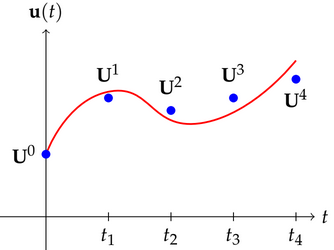
\includegraphics[height=0.6\textheight, width=0.6\textwidth, keepaspectratio]{./Images/approximation_08.png}
	\end{center}
\end{figure}

Para obter este método, consideraremos a expansão em série de Taylor em torno de \(t_{n}\) para u:
\[
	\mathbf{u}(t_{n}+h) = \mathbf{u}(t_{n}) + h \mathbf{u}'(t_{n}) + \underbrace{\frac{h^{2}}{2}\mathbf{u}''(t_{n})+\dotsc +\frac{h^{q}}{q!}\mathbf{u}^{(q)}(t_{n})}_{= \mathcal{O}(h^{2})}+\dotsc .
\]

\begin{def*}
	Dizemos que \(\mathbf{g}(h)\) é da \textbf{ordem de \(\mathbf{h^{p}}\)}, ou seja, é \(\mathbf{\mathcal{O}(h^{p})}\), se existe uma constante \(C> 0\) independente de h, tal que, para todo h suficientemente pequeno,
	\[
		\biggl\Vert \frac{\mathbf{g}(h)}{h^{p}} \biggr\Vert \leq C. \; \square
	\]
\end{def*}
Note que tanto a função \(\mathbf{u}(t)\) quanto as suas derivadas não são conhecidas, mas podemos usar a condição \(\mathbf{u}'(t) = \mathbf{f}(\mathbf{u}(t), t)\) para obter
\[
	\mathbf{u}(t_{n}+h) = \mathbf{u}(t_{n}) + h \mathbf{u}'(t_{n}) + \mathcal{O}(h^{2}) = \mathbf{u}(t_{n}) + h \mathbf{f}(\mathbf{u}(t_{n}), t_{n}) + \mathcal{O}(h^{2}).
\]
Assim, podemos gerar uma aproximação para a solução do PVI original ao descartarmos os termos \(\mathcal{O}(h^{2})\), resultando no \textbf{método de Euler}
\[
	\boxed{\mathbf{U}^{n+1} = \mathbf{U}^{n} + h \mathbf{f}(\mathbf{U}^{n}, t_{n})}.
\]
Como o últimos termo que sobrevive corresponde a \(q=1\) na expansão, este método também é conhecido como \textbf{método de Taylor de ordem q = 1}.

\begin{example}
	Para aproximar o PVI
	\[
		\left\{\begin{array}{ll}
			y'(x) = x + y, \quad x\in [0, 1] \\
			y(0) = \frac{1}{2}
		\end{array}\right.
	\]
	usando o método de Euler com \(h=\frac{1}{10}\), começamos observando que a forma da função, aqui, é
	\[
		f(y(x), x) = x+y;
	\]
	como \(h = \frac{1}{10},\) temos \(x_{0} = 0,\; x_1 = \frac{1}{10},\; x_2 = \frac{2}{10} = \frac{1}{5}, \dotsc , x_10 = \frac{10}{10}=1\), de forma que
	\begin{align*}
		 & Y^{0} = y(0) = \frac{1}{2}                                                                                                              \\
		 & Y^{1} = Y^{0}+hf(Y^{0}, x_{0}) = \frac{1}{2}+hf\biggl(\frac{1}{2}, 0\biggr)= \frac{1}{2}+\frac{1}{10}\frac{1}{2} = \frac{11}{20} = 0.55 \\
		 & Y^{2} = Y^{1} + h f(Y^{1}, x_1) = \frac{11}{20}+hf\biggl(\frac{11}{20}, \frac{1}{10}\biggr) = \frac{123}{200} = 0.615                   \\
		 & \vdots
	\end{align*}
	resultando na tabela
	\begin{table}[H]
		\centering
		\caption{Método de Euler com 10 pontos}
		\begin{tabular}{| c | c | c |}
			\hline
			x   & \(Y^{n}\) & \(E^{n}\) \\
			\hline
			0.0 & 0.500000  & 0.0       \\
			0.1 & 0.550000  & 0.007756  \\
			0.2 & 0.615000  & 0.017104  \\
			0.3 & 0.696500  & 0.028288  \\
			0.4 & 0.796150  & 0.041587  \\
			0.5 & 0.915765  & 0.057316  \\
			0.6 & 1.057341  & 0.075836  \\
			0.7 & 1.223075  & 0.097553  \\
			0.8 & 1.415383  & 0.122928  \\
			0.9 & 1.636921  & 0.152483  \\
			1.0 & 1.890613  & 0.186809  \\
			\hline
		\end{tabular}
	\end{table}
	A solução exata é
	\[
		y(x) = \frac{3}{2}e^{x}-x-1,
	\]
	e o erro é
	\[
		E^{n} = y(x_{n})-Y^{n}
	\]
\end{example}

\begin{example}[Pêndulo, parte 2]
	Vamos escrever o método de Euler para aproximar o problema do pêndulo: primeiramente, lembre-se da forma final do problema do pêndulo:
	\[
		\left\{\begin{array}{ll}
			\mathbf{u}'(t) = \mathbf{f}(\mathbf{u}(t), t) \\
			\mathbf{u}(0) = \mathbf{u}_{0},
		\end{array}\right.
	\]
	onde
	\begin{align*}
		 & \mathbf{u}(t) = \begin{bmatrix}
			                   u_1(t) \\
			                   u_2(t)
		                   \end{bmatrix},                 \\
		 & \mathbf{f}(\mathbf{u}(t), t) = \begin{bmatrix}
			                                  u_2(t) \\
			                                  -\sin^{}{u_1(t)}
		                                  \end{bmatrix}, \\
		 & \mathbf{u}^{0} = \begin{bmatrix}
			                    q^{0} \\
			                    p^{0}
		                    \end{bmatrix},
	\end{align*}
	tal que
	\[
		\mathbf{U}^{n+1} = \mathbf{U}^{n} + h \mathbf{f}(\mathbf{U}^{n}, t_{n}) \Rightarrow \begin{bmatrix}
			U_{1}^{n+1} \\
			U_{2}^{n+1}
		\end{bmatrix} = \begin{bmatrix}
			U_{1}^{n} \\
			U_{2}^{n}
		\end{bmatrix} + h \begin{bmatrix}
			U_{2}^{n} \\
			-\sin^{}{(U_{1}^{n})}
		\end{bmatrix}
	\]
\end{example}

Em outras situações, será desejável obter uma aproximação de Taylor de ordem \(q=2\); para isso, olhamos para mesma expansão de antes:
\[
	\mathbf{u}(t_{n}+h) = \mathbf{u}(t_{n}) + h \mathbf{u}'(t_{n}) + \frac{h^{2}}{2}\mathbf{u}''(t_{n}) \underbrace{+\dotsc +\frac{h^{q}}{q!}\mathbf{u}^{(q)}(t_{n})}_{= \mathcal{O}(h^{3})}+\dotsc,
\]
e substituímos nela as derivadas de \(\mathbf{u}\) em termos de \(\mathbf{f}\):
\[
	\mathbf{u}'(t_{n}) = \mathbf{f}(\mathbf{u}(t_{n}), t_{n})
\]
e
\begin{align*}
	\mathbf{u}''(t_{n}) = \frac{\mathrm{d}}{\mathrm{d}t}\mathbf{f}(\mathbf{u}(t_{n}), t) & = \frac{\partial^{}\mathbf{f}}{\partial \mathbf{u}^{}}\biggl|_{(\mathbf{u}(t_{n}), t_{n})}^{}\biggr. \frac{\mathrm{d}\mathbf{u}}{\mathrm{d}t}\biggl|_{t_{n}}^{}\biggr. + \frac{\partial^{}\mathbf{f}}{\partial t^{}}\biggl|_{(\mathbf{u}(t_{n}), t_{n})}^{}\biggr. \frac{\mathrm{d}t}{\mathrm{d}t}\biggl|_{t_{n}}^{}\biggr. \\
	                                                                                     & =\biggl(\frac{\partial^{}\mathbf{f}}{\partial \mathbf{u}^{}} f + \frac{\partial^{}\mathbf{f}}{\partial t^{}}\biggr)\biggl|_{(\mathbf{u}(t_{n}), t_{n})}^{}\biggr.,
\end{align*}
onde o termo \(\displaystyle \frac{\partial^{}\mathbf{f}}{\partial \mathbf{u}^{}}\) é uma notação para a matriz Jacobiana de f, dada por
\[
	\frac{\partial^{}\mathbf{f}}{\partial \mathbf{u}^{}} = \begin{bmatrix}
		\frac{\partial^{}f_1}{\partial u_1^{}} & \frac{\partial^{}f_1}{\partial u_2^{}} & \dotsc & \frac{\partial^{}f_1}{\partial u_{m}^{}} \\
		\frac{\partial^{}f_2}{\partial u_1^{}} & \frac{\partial^{}f_2}{\partial u_2^{}} & \dotsc & \frac{\partial^{}f_2}{\partial u_{m}^{}} \\
		\vdots                                 & \vdots                                 & \ddots & \vdots                                   \\
		\frac{\partial^{}f_m}{\partial u_1^{}} & \frac{\partial^{}f_m}{\partial u_2^{}} & \dotsc & \frac{\partial^{}f_m}{\partial u_{m}^{}}
	\end{bmatrix} = \biggl(\frac{\partial^{}f_{i}}{\partial u_{j}^{}}\biggr)_{ij}.
\]
Daí, destacando os termos \(\mathcal{O}(h^{3})\) da série de Taylor, chega-se na fórmula discreta do método:
\[
	\mathbf{U}^{n+1} = \mathbf{U}^{n} + h \mathbf{f}(\mathbf{U}^{n}, t_{n}) + \frac{h^{2}}{2}\biggl(\frac{\partial^{}\mathbf{f}}{\partial \mathbf{u}^{}}\mathbf{f} + \frac{\partial^{}\mathbf{f}}{\partial t^{}}\biggr)\biggl|_{(\mathbf{U}^{n}, t_{n})}^{}\biggr.
\]
\begin{example}
	Vamos revisitar o exemplo
	\[
		\left\{\begin{array}{ll}
			y'(x) = x + y, \quad x\in [0, 1] \\
			y(0) = \frac{1}{2}
		\end{array}\right.,
	\]
	mas com o método de Taylor de ordem \(q=2\) -- no método escalar, com \(m=1\), ela se reduz a
	\[
		U^{m+1} = U^{m} + h f(U^{n}, t_{n}) _ \frac{h^{2}}{2}\biggl(\frac{\partial^{}f}{\partial u^{}}f + \frac{\partial^{}f}{\partial t^{}}\biggr)\biggl|_{(U^{n}, t_{n})}^{}\biggr.,
	\]
	e, adequando-se à notação utilizada, temos
	\[
		f(y(x), x) = x+y,\quad \frac{\partial^{}f}{\partial y^{}}(y(x), x) = 1,\quad \frac{\partial^{}f}{\partial x^{}} = 1,
	\]
	de modo que, para este exemplo,
	\[
		Y^{n+1} = Y^{n} + h f(Y^{n}, x_{n}) + \frac{h^{2}}{2}(f(Y^{n}, x_{n})+1),
	\]
	e podemos comparar as tabelas com ordens distintas:

	\begin{table}[H]
		\centering
		\caption{Método de Euler com 10 pontos}
		\begin{tabular}{| c | c | c | c | c |}
			\hline
			\multirow{ 2}{*}{x} & \multicolumn{2}{c |}{Taylor q = 1} & \multicolumn{2}{c |}{Taylor q = 2}                         \\
			                    & \(Y^{n}\)                          & \(E^{n}\)                          & \(Y^{n}\) & \(E^{n}\) \\
			\hline
			0.0                 & 0.500000                           & 0.000000                           & 0.500000  & 0.000000  \\
			0.1                 & 0.550000                           & 0.007756                           & 0.557500  & 0.000256  \\
			0.2                 & 0.615000                           & 0.017104                           & 0.631537  & 0.000566  \\
			0.3                 & 0.696500                           & 0.028288                           & 0.723848  & 0.000939  \\
			0.4                 & 0.796150                           & 0.041587                           & 0.836353  & 0.001383  \\
			0.5                 & 0.915765                           & 0.057316                           & 0.971170  & 0.001911  \\
			0.6                 & 1.057341                           & 0.075836                           & 1.130643  & 0.002535  \\
			0.7                 & 1.223075                           & 0.097553                           & 1.317360  & 0.003268  \\
			0.8                 & 1.415383                           & 0.122928                           & 1.534183  & 0.004128  \\
			0.9                 & 1.636921                           & 0.152483                           & 1.784272  & 0.005132  \\
			1.0                 & 1.890613                           & 0.186809                           & 2.071121  & 0.006301  \\
			\hline
		\end{tabular}
	\end{table}
\end{example}
\begin{example}[Pêndulo, parte 3]
	Agora, para resolver o problema do pêndulo do exemplo 2 usando o método de Taylor de ordem \(q=2\), consideramos
	\[
		\mathbf{f}(\mathbf{u}(t), t) = \begin{bmatrix}
			u_2(t) \\
			-\sin^{}{u_1(t)}
		\end{bmatrix}
	\]
	e calculamos
	\[
		\frac{\partial^{}\mathbf{f}}{\partial t^{}}=\begin{bmatrix}
			0 \\
			0
		\end{bmatrix}, \quad \frac{\partial^{}\mathbf{f}}{\partial \mathbf{u}^{}}=\begin{bmatrix}
			\frac{\partial f_1}{\partial u_1^{}}   & \frac{\partial^{}f_1}{\partial u_2^{}} \\
			\frac{\partial^{}f_2}{\partial u_1^{}} & \frac{\partial^{}f_2}{\partial u_2^{}}
		\end{bmatrix} = \begin{bmatrix}
			0               & 1 \\
			-\cos^{}{(u_1)} & 0
		\end{bmatrix}.
	\]
	Portanto, o método fica
	\[
		\begin{bmatrix}
			U_{1}^{n+1} \\
			U_{2}^{n+1}
		\end{bmatrix} = \begin{bmatrix}
			U_{1}^{n} \\
			U_{2}^{n}
		\end{bmatrix} + h \begin{bmatrix}
			U_{2}^{n} \\
			- \sin^{}{(U_{1}^{n})}
		\end{bmatrix} + \frac{h^{2}}{2} \begin{bmatrix}
			0                     & 1 \\
			-\cos^{}{(U_{1}^{n})} & 0
		\end{bmatrix} \begin{bmatrix}
			U_{2}^{n} \\
			-\sin^{}{(U_{1}^{n})}
		\end{bmatrix},
	\]
	ou ainda, em forma de sistemas,
	\[
		\left\{\begin{array}{ll}
			U_{1}^{n+1} = U_{1}^{n} + h U_{2}^{n} - \frac{h^{2}}{2}\sin^{}{(U_{1}^{n})} \\
			U_{2}^{n+1} = U_{2}^{n} - h \sin^{}{(U_{1}^{n})} - \frac{h^{2}}{2}U_{2}^{n}\cos^{}{(U_{1}^{n})}
		\end{array}\right..
	\]
	Como se comparam as aproximações? Basta olhar as tabelas de antes e as imagens a seguir:
	\begin{figure}[H]
		\begin{center}
			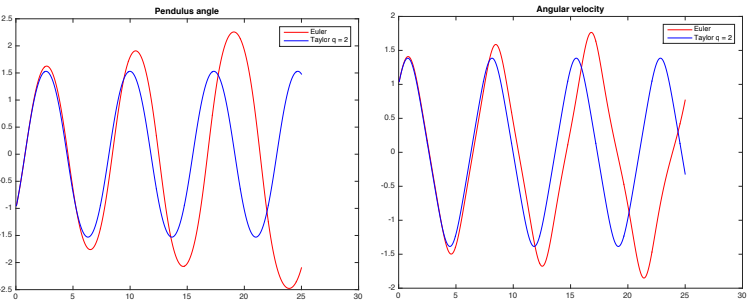
\includegraphics[height=\textheight, width=\textwidth, keepaspectratio]{./Images/pendulus_08.png}
		\end{center}
	\end{figure}
\end{example}

Vamos nos restringir ao caso escalar e obter aproximações de Taylor de ordens superiores:
\[
	u(t_{n}+h) = u(t_{n}) + h u'(t_{n}) = \frac{h^{2}}{2}u''(t_{n}) + \frac{h^{3}}{6}h'''(t_{n}) + \mathcal{O}(h^{4}),
\]
tal que, derivando,
\begin{align*}
	 & \tikz[baseline=-0.5ex]\draw[black, fill=black, radius=1.5pt](0, 0)circle;\; u'(t_{n}) = f(u(t_{n}), t_{n})                                                                                                              \\
	 & \tikz[baseline=-0.5ex]\draw[black, fill=black, radius=1.5pt](0, 0)circle;\; (f_{u}f + f_{t})\biggl|_{(u(t_{n}), t_{n})}^{}\biggr.                                                                                       \\
	 & \tikz[baseline=-0.5ex]\draw[black, fill=black, radius=1.5pt](0, 0)circle;\; u'''(t_{n}) = \frac{\mathrm{d}}{\mathrm{d}t}u''(t_{n}) = \frac{\mathrm{d}}{\mathrm{d}t}(f_{u}f + f_{t}\biggl|_{(u(t_{n}), t_{n})}^{}\biggr. \\
	 & \quad\; \quad \quad = [(f_{uu}f + f_{ut}) + (f_u f + f_{t})f_u + (f_{tu}f + f_{tt})]\biggl|_{u(t_{n}), t_{n}}^{}\biggr.                                                                                                 \\
	 & \quad\; \quad \quad = [(f_{uu}f + f_{ut}) + (f_u f + f_{t})f_u + (f_{tu}f + f_{tt})]\biggl|_{u(t_{n}), t_{n}}^{}\biggr.                                                                                                 \\
\end{align*}

\begin{tcolorbox}[
		skin=enhanced,
		title=Observação,
		fonttitle=\bfseries,
		colframe=black,
		colbacktitle=cyan!75!white,
		colback=cyan!15,
		colbacklower=black,
		coltitle=black,
		drop fuzzy shadow,
		%drop large lifted shadow
	]
	É importante fazer algumas observações referentes ao método de Taylor -- a precisão do método aumenta com q, mas a complexidade dos cálculos aumenta \textit{bastante} para q maior que 3; apesar disso, é possível implementar métodos de Taylor de ordens superiores, inclusive para sistemas, fazendo diferenciações ``espertas'' diretamente no código.

	A maior desvantagem disso é que ele exige diferenciabilidade de \(\mathbf{f}\), que não é uma condição para a existência de uma solução e, consequentemente, o método não pode ser aplicado para problemas onde \(\mathbf{f}\) perde suavidade.
\end{tcolorbox}
\begin{listing}[H]
	\caption{Implementação de Taylor de ordem q para o pêndulo}
	\begin{minted}[bgcolor = bg, linenos=true, breaklines]{matlab}
  function fd = fandd(t, y) 

  % linhas - ordem da derivada + 1 
  % colunas - numero da equacao 
  
  fd(1, 1) = y(2); 
  fd(1, 2) = -sin(y(1)); 

  fd(2, 1) = fd(1, 2); 
  fd(2, 2 ) = -cos(y(1))*fd(1, 1); 

  fd(3, 1) = fd(2, 2); 
  fd(3, 2) = fd(1, 1)*sin(y(1))*fd(1, 1) - cos(y(1))*fd(2, 1)
\end{minted}
\end{listing}
\end{document}
